\section{Results}\label{sec:results}
% \tikzexternalenable

Results were obtained with \gls{hms} using the \gls{frozen-block-LTS} scheme including neighbor propagation and the revised criterion for scalar flux computations covered in \autoref{sec:mods}.

% \note{anything about the computer used for these results?}

\subsection{1D Dam Break} 

\subsubsection{Accuracy} \label{sec:results-accuracy-analytical}

The \gls{1D} dam break was used for validating the implemented \gls{frozen-block-LTS} scheme.
\autoref{fig:acc-fo} and \autoref{fig:acc-tvd} show water depth and velocity profiles for both wet and dry dam break cases at time $t=\SI{0.6}{\second}$ using first-order and \gls{tvd} reconstruction, respectively.
\gls{gts} values are represented by circle marks,
\gls{lts} values are shown as cross marks,
and the analytical solution is drawn as a solid black line.
% Since
Visually, no differences between the numerical results can be identified.
% A visual analysis does not show any differences between values obtained through \gls{gts} and \gls{lts}, as both marks align perfectly in all cases. 
This applies to both first-order and \gls{tvd} reconstruction.

\autoref{tab:nse-accuracy} contains \gls{nse} results of the \gls{1D} dam break.
Similarly to the plots, they do not indicate a loss of accuracy through the use of the \gls{lts} scheme.
For both water depth and velocity using \gls{tvd} reconstruction, as well as water depth with first-order reconstruction,
the first six decimal places 
% of the \gls{nse} 
are identical between the \gls{gts} and \gls{lts} schemes.
Only the \gls{nse} for the velocity in the case of first-order reconstruction exhibits any difference between the time-stepping schemes:
In the wet case, the difference is only \num{1e-6}, while the largest difference in \gls{nse} is observed in the dry case, where it amounts to $<\num{2e-4}$. Both can be considered negligible.
% For \gls{tvd} reconstruction, the \gls{nse} does not differ between \gls{gts} and \gls{lts} solutions at all until the sixth decimal place.
% For the first-order reconstruction scheme, there are no differences in the water depth's \gls{nse}.
% Although the velocity's \gls{nse} differs slightly for both cases, for the wet case, it is by just $\num{1e-6}$, and for the dry case by $\num{1.73e-4}$; both can be considered negligible.

\begin{table}[!h]
  \caption
  [\acrshort{nse} for the 1D dam break cases]
  {
    \acrshort{nse} of water depth $d$ and velocity $u$ at time $t=\SI{0.6}{\second}$ for wet and dry \acrshort{1D} dam break cases, using both first-order and \acrshort{tvd} reconstruction.
  }
  \label{tab:nse-accuracy}
  \small
  \centering
  \sisetup{
  table-format=1.6,
}

\begin{tabular}{rc*{2}{S[round-precision=6, round-mode=places]}c*{2}{S[round-precision=6, round-mode=places]}} 
  \toprule
  &  & \multicolumn{2}{c}{first-order reconstruction} & & \multicolumn{2}{c}{\gls{tvd} reconstruction} \\
  \cmidrule(r){3-4} \cmidrule(r){6-7}
          &  & {\gls{gts}} & {\gls{lts}} &  & {\gls{gts}} & {\gls{lts}} \\
  \midrule
  $d$ wet &  & 0.998121725 & 0.998121745 &  & 0.999048143 & 0.999048143 \\
  $v$ wet &  & 0.989963481 & 0.989963645 &  & 0.993198985 & 0.993198985 \\
  \midrule
  $d$ dry &  & 0.999629393 & 0.999629424 &  & 0.999974986 & 0.999974987 \\
  $v$ dry &  & 0.849061523 & 0.848888537 &  & 0.962224377 & 0.962224377 \\
  \bottomrule
\end{tabular}
\end{table}

However, in the wet dam break cases, only \SI{0.22}{\percent} of all flux updates are scalar computations.
This is due to the small cell sizes of this scenario, see \autoref{sec:results-benchmarks}.
Therefore, the relevance of this test configuration, as well as its results, may be questioned.
The impact of cell size is further analyzed in \autoref{sec:results-benchmarks}.
The heatmaps below the water depth and velocity profiles illustrate the \gls{ssc}:
lighter colors indicate a lighter load, i.e., a higher \acrlong{ssc}, while darker colors denote more full flux computations.
% light blocks are often updated using scalar flux computations, dark blocks used full flux computations for all updates.

\begin{figure}[htbp]
  \centering

  \begin{subfigure}{\textwidth}
  \centering
  \begin{tikzpicture}
    \begin{axis}[
        % title={Wet Dambreak Case using first-order reconstruction},
        xlabel={$x \ [\si{\meter}]$},
        ylabel={$d [\si{\meter}]$},
        % ymin=-0.5,
        legend pos=north east,
        % ymajorgrids=true,
        % grid style=loosely dashed,
      ]
      % analytical
      \addplot [black, very thin, mark=none] 
        table [x=x, y=d_ana, col sep=comma] {./graphs/accuracy/data/wet_t0.6s.csv};
      % GTS
      \addplot [only marks, lightgray, mark=o, mark repeat=5, mark phase=1] 
        table [x=x, y=d_gts_fo, col sep=comma] {./graphs/accuracy/data/wet_t0.6s.csv};
      % LTS
      \addplot [only marks, CadetBlue, mark=x, mark repeat=5, mark phase=1] 
        table [x=x, y=d_lts_fo, col sep=comma] {./graphs/accuracy/data/wet_t0.6s.csv};
      \legend{analytical, GTS, LTS}
    \end{axis}
  \end{tikzpicture}
  \hfill
  \begin{tikzpicture}
    \begin{axis}[
        % title={Wet Dambreak Case using first-order reconstruction},
        xlabel={$x \ [\si{\meter}]$},
        ylabel={$v \ [\si{\meter\per\second}]$},
        % ymin=-0.5,
        legend pos=north west,
        % ymajorgrids=true,
        % grid style=loosely dashed,
      ]
      % analytical
      \addplot [black, very thin, mark=none] 
        table [x=x, y=v_ana, col sep=comma] {./graphs/accuracy/data/wet_t0.6s.csv};
      % GTS
      \addplot [only marks, lightgray, mark=o, mark repeat=5, mark phase=1] 
        table [x=x, y=v_gts_fo, col sep=comma] {./graphs/accuracy/data/wet_t0.6s.csv};
      % LTS
      \addplot [only marks, CadetBlue, mark=x, mark repeat=5, mark phase=1] 
        table [x=x, y=v_lts_fo, col sep=comma] {./graphs/accuracy/data/wet_t0.6s.csv};
      \legend{analytical, GTS, LTS}
    \end{axis}
  \end{tikzpicture}
  \\ \vspace{0.4cm}
  \includegraphics[width=0.8\textwidth]{../typst/heatmaps/analytical/dambreak_wet_lts_fo.pdf}
  \\ \vspace{0.4cm}
  \caption{Wet dam break}\label{fig:acc-wet-fo}
\end{subfigure}

\vspace{1cm}

\begin{subfigure}{\textwidth}
  \centering
  \begin{tikzpicture}
    \begin{axis}[
        % title={Wet Dambreak Case using first-order reconstruction},
        xlabel={$x \ [\si{\meter}]$},
        ylabel={$d [\si{\meter}]$},
        % ymin=-0.5,
        legend pos=north east,
        % ymajorgrids=true,
        % grid style=loosely dashed,
      ]
      % analytical
      \addplot [black, very thin, mark=none] 
        table [x=x, y=d_ana, col sep=comma] {./graphs/accuracy/data/dry_t0.6s.csv};
      % GTS
      \addplot [only marks, lightgray, mark=o, mark repeat=5, mark phase=1] 
        table [x=x, y=d_gts_fo, col sep=comma] {./graphs/accuracy/data/dry_t0.6s.csv};
      % LTS
      \addplot [only marks, CadetBlue, mark=x, mark repeat=5, mark phase=1] 
        table [x=x, y=d_lts_fo, col sep=comma] {./graphs/accuracy/data/dry_t0.6s.csv};
      \legend{analytical, GTS, LTS}
    \end{axis}
  \end{tikzpicture}
  \hfill
  \begin{tikzpicture}
    \begin{axis}[
        xlabel={$x \ [\si{\meter}]$},
        ylabel={$v \ [\si{\meter\per\second}]$},
        % ymin=-0.5,
        legend pos=north west,
        % ymajorgrids=true,
        % grid style=loosely dashed,
      ]
      % analytical
      \addplot [black, very thin, mark=none] 
        table [x=x, y=v_ana, col sep=comma] {./graphs/accuracy/data/dry_t0.6s.csv};
      % GTS
      \addplot [only marks, lightgray, mark=o, mark repeat=5, mark phase=4] 
        table [x=x, y=v_gts_fo, col sep=comma] {./graphs/accuracy/data/dry_t0.6s.csv};
      % LTS
      \addplot [only marks, CadetBlue, mark=x, mark repeat=5, mark phase=4] 
        table [x=x, y=v_lts_fo, col sep=comma] {./graphs/accuracy/data/dry_t0.6s.csv};
      \legend{analytical, GTS, LTS}
    \end{axis}
  \end{tikzpicture}
  \\ \vspace{0.4cm}
  \includegraphics[width=0.8\textwidth]{../typst/heatmaps/analytical/dambreak_dry_lts_fo.pdf}
  \\ \vspace{0.4cm}
  \caption{Dry dam break}\label{fig:acc-dry-fo}
\end{subfigure}

  \caption
  [Water depth and velocity profiles for the 1D dam break case, with heatmaps, first-order reconstruction]
  {
    Water depth and velocity profiles at time $t=\SI{0.6}{\second}$ for wet and dry \acrshort{1D} dam break cases using first-order reconstruction, with heat maps illustrating the \acrshort{ssc}.
  }
  \label{fig:acc-fo}
\end{figure}

\begin{figure}[htbp]
  \centering

  \begin{subfigure}{\textwidth}
  \centering
  \begin{tikzpicture}
    \begin{axis}[
        xlabel={$x \ [\si{\meter}]$},
        ylabel={$d [\si{\meter}]$},
        % ymin=-0.5,
        legend pos=north east,
        % ymajorgrids=true,
        % grid style=loosely dashed,
      ]
      % analytical
      \addplot [black, very thin, mark=none] 
        table [x=x, y=d_ana, col sep=comma] {./graphs/accuracy/data/wet_t0.6s.csv};
      % GTS
      \addplot [only marks, lightgray, mark=o, mark repeat=5, mark phase=1] 
        table [x=x, y=d_gts_tvd, col sep=comma] {./graphs/accuracy/data/wet_t0.6s.csv};
      % LTS
      \addplot [only marks, CadetBlue, mark=x, mark repeat=5, mark phase=1] 
        table [x=x, y=d_lts_tvd, col sep=comma] {./graphs/accuracy/data/wet_t0.6s.csv};
      \legend{analytical, GTS, LTS}
    \end{axis}
  \end{tikzpicture}
  \hfill
  \begin{tikzpicture}
    \begin{axis}[
        xlabel={$x \ [\si{\meter}]$},
        ylabel={$v \ [\si{\meter\per\second}]$},
        % ymin=-0.5,
        legend pos=north west,
        % ymajorgrids=true,
        % grid style=loosely dashed,
      ]
      % analytical
      \addplot [black, very thin, mark=none] 
        table [x=x, y=v_ana, col sep=comma] {./graphs/accuracy/data/wet_t0.6s.csv};
      % GTS
      \addplot [only marks, lightgray, mark=o, mark repeat=5, mark phase=1] 
        table [x=x, y=v_gts_tvd, col sep=comma] {./graphs/accuracy/data/wet_t0.6s.csv};
      % LTS
      \addplot [only marks, CadetBlue, mark=x, mark repeat=5, mark phase=1] 
        table [x=x, y=v_lts_tvd, col sep=comma] {./graphs/accuracy/data/wet_t0.6s.csv};
      \legend{analytical, GTS, LTS}
    \end{axis}
  \end{tikzpicture}
  \\ \vspace{0.4cm}
  \includegraphics[width=0.8\textwidth]{../typst/heatmaps/analytical/dambreak_wet_lts_tvd.pdf}
  \\ \vspace{0.4cm}
  \caption{Wet dam break}\label{fig:acc-wet-tvd}
\end{subfigure}

\vspace{1cm}

\begin{subfigure}{\textwidth}
  \centering
  \begin{tikzpicture}
    \begin{axis}[
        xlabel={$x \ [\si{\meter}]$},
        ylabel={$d [\si{\meter}]$},
        % ymin=-0.5,
        legend pos=north east,
        % ymajorgrids=true,
        % grid style=loosely dashed,
      ]
      % analytical
      \addplot [black, very thin, mark=none] 
        table [x=x, y=d_ana, col sep=comma] {./graphs/accuracy/data/dry_t0.6s.csv};
      % GTS
      \addplot [only marks, lightgray, mark=o, mark repeat=5, mark phase=1] 
        table [x=x, y=d_gts_tvd, col sep=comma] {./graphs/accuracy/data/dry_t0.6s.csv};
      % LTS
      \addplot [only marks, CadetBlue, mark=x, mark repeat=5, mark phase=1] 
        table [x=x, y=d_lts_tvd, col sep=comma] {./graphs/accuracy/data/dry_t0.6s.csv};
      \legend{analytical, GTS, LTS}
    \end{axis}
  \end{tikzpicture}
  \hfill
  \begin{tikzpicture}
    \begin{axis}[
        xlabel={$x \ [\si{\meter}]$},
        ylabel={$v \ [\si{\meter\per\second}]$},
        % ymin=-0.5,
        legend pos=north west,
        % ymajorgrids=true,
        % grid style=loosely dashed,
      ]
      % analytical
      \addplot [black, very thin, mark=none] 
        table [x=x, y=v_ana, col sep=comma] {./graphs/accuracy/data/dry_t0.6s.csv};
      % GTS
      \addplot [only marks, lightgray, mark=o, mark repeat=5, mark phase=4] 
        table [x=x, y=v_gts_tvd, col sep=comma] {./graphs/accuracy/data/dry_t0.6s.csv};
      % LTS
      \addplot [only marks, CadetBlue, mark=x, mark repeat=5, mark phase=4] 
        table [x=x, y=v_lts_tvd, col sep=comma] {./graphs/accuracy/data/dry_t0.6s.csv};
      \legend{analytical, GTS, LTS}
    \end{axis}
  \end{tikzpicture}
  \\ \vspace{0.4cm}
  \includegraphics[width=0.8\textwidth]{../typst/heatmaps/analytical/dambreak_dry_lts_tvd.pdf}
  \\ \vspace{0.4cm}
  \caption{Dry dam break}\label{fig:acc-dry-tvd}
\end{subfigure}

  \caption
  [Water depth and velocity profiles for the 1D dam break case, with heatmaps, TVD reconstruction]
  {
    Water depth and velocity profiles at time $t=\SI{0.6}{\second}$ for wet and dry \acrshort{1D} dam break cases using \acrshort{tvd} reconstruction, with heat maps illustrating the \acrshort{ssc}.
  }
  \label{fig:acc-tvd}
\end{figure}

\FloatBarrier
\newpage
\FloatBarrier
\subsubsection{Runtime Analysis}\label{sec:results-benchmarks}

In the dam break cases for runtime benchmarks, a collection of variants has been introduced, see \autoref{sec:case-dambreak}.
Every variant has been run 25 times for each combination of \gls{gts}/\gls{lts} first-order/\gls{tvd} reconstruction.
\autoref{tab:benchmarks} lists the average runtime of these runs, the relative difference between \gls{gts} and \gls{lts} runtimes as \gls{rtr} and \acrfull{ssc}.
Variations were considered negligible, as standard deviations are $< \SI{1}{\percent}$ of the average values for all configurations, except for the reduced block size of $8 \times 8$ cells, where it amounts to $\sim\!\SI{2}{\percent}$.

The base configuration shows that runtime can be reduced by \SI{10.09}{\percent} through \gls{lts} for first-order and by \SI{12.05}{\percent} for \gls{tvd} reconstruction.
Other configurations have shown both higher and lower reduction values.
While decreasing block size from $64 \times 64$ to $32 \times 32$ showed an increased reduction, setting it to $8 \times 8$ and $128 \times 128$ showed a decrease in runtime reduction.
This indicates that there is an optimal value for this parameter for the use of \gls{frozen-block-LTS} somewhere between $8 \times 8$ and $64 \times 64$, possibly, close to $32 \times 32$.

\begin{table}[!h]
  \caption{
    Average runtime of 25 runs, with \acrfull{rtr} and \acrfull{ssc} for the selected dam break cases.
  }
  \label{tab:benchmarks}
  \small
  \begin{adjustbox}{center}
  \sisetup{
  table-format=1.1,
}

\addtolength{\tabcolsep}{-3pt}
\begingroup
\begin{tabular}{
  r
  % *{2}{S[round-mode=places,round-precision=2,table-space-text-post={\,s}]<{\,s}}
  % *{2}{S[round-mode=places,round-precision=1,table-format=2.1,table-space-text-post={\,\%}]<{\,\%}}
  % *{2}{S[round-mode=places,round-precision=2,table-space-text-post={\,s}]<{\,s}}
  % *{2}{S[round-mode=places,round-precision=1,table-format=2.1,table-space-text-post={\,\%}]<{\,\%}}
  *{2}{S[round-mode=places,round-precision=1]}
  *{2}{S[round-mode=places,round-precision=1,table-format=2.1]}
  *{2}{S[round-mode=places,round-precision=1]}
  *{2}{S[round-mode=places,round-precision=1,table-format=2.1]}
  }

  \toprule
  &  \multicolumn{4}{c}{first-order reconstruction} & \multicolumn{4}{c}{\gls{tvd} reconstruction} \\
  \cmidrule(r){2-5} \cmidrule(r){6-9}

  % var0-base-dambreak_wet_0.6s_64x64_2000_gts_fo

  % {Benchmark variant}                        & \mc{\gls{gts}}     & \mc{\gls{lts}}     & \mc{\acrshort{rtr}} & \mc{\acrshort{ssc}} & \mc{\gls{gts}}     & \mc{\gls{lts}}      & \mc{\acrshort{rtr}} & \mc{\acrshort{ssc}} \\
  {Benchmark variant}                        & \mc{\gls{gts}\,[\si\second]} & \mc{\gls{lts}\,[\si\second]} & \mc{\acrshort{rtr}\,[\si\percent]} & \mc{\acrshort{ssc}\,[\si\percent]} & \mc{\gls{gts}\,[\si\second]} & \mc{\gls{lts}\,[\si\second]} & \mc{\acrshort{rtr}\,[\si\percent]} & \mc{\acrshort{ssc}\,[\si\percent]} \\
  \midrule
  base configuration                         & 1.2252                        & 1.1016000000000001            & 10.09                               & 15.679253472222221                  & 1.7600400000000003            & 1.54792                       & 12.05                               & 15.729527104959631                  \\
  block size $8 \times 8$                    & 2.47716                       & 2.25036                       & 9.16                                & 16.401777777777777                  & 3.3421200000000004            & 3.02072                       & 9.62                                & 16.469216287337982                  \\
  block size $32 \times 32$                  & 1.1273600000000001            & 1.03392                       & 8.29                                & 14.800347222222221                  & 1.6399999999999997            & 1.4624400000000002            & 10.83                               & 14.917695473251028                  \\
  block size $128 \times 128$                & 1.3928                        & 1.23364                       & 11.43                               & 15.894011925757958                  & 1.93716                       & 1.6939199999999999            & 12.56                               & 15.914529914529915                  \\
  mesh size $1000 \times 1000$               & 4.86012                       & 4.34656                       & 10.57                               & 15.894011925757958                  & 6.955160000000001             & 6.10768                       & 12.18                               & 15.913214990138066                  \\
  mesh size $4000 \times 4000$               & 0.309892                      & 0.279612                      & 9.77                                & 14.800347222222221                  & 0.449192                      & 0.39963600000000005           & 11.03                               & 14.951989026063101                  \\
  $t_{\text{end}}= \SI{6.0}{\second}$        & 2.44272                       & 2.17816                       & 10.83                               & 15.65212673611111                   & 3.5118                        & 3.0832800000000002            & 12.20                               & 15.710303729334871                  \\
  $l_x = l_y = \SI{0.5}{\meter}$             & 2.3056                        & 2.19536                       & 4.78                                & 8.208869485294118                   & 3.3236399999999997            & 3.16484                       & 4.78                                & 6.95857927946265                    \\
  $l_x = l_y = \SI{2.0}{\meter}$             & 0.819804                      & 0.683752                      & 16.60                               & 23.53515625                         & 1.1768800000000001            & 0.9588239999999999            & 18.53                               & 23.673587081891583                  \\
  $\Cr = 0.1$                                & 3.0488399999999998            & 2.99996                       & 1.60                                & 4.1796875                           & 4.48292                       & 4.42332                       & 1.33                                & 3.0803369941326912                  \\
  $\Cr = 0.5$                                & 0.8186240000000001            & 0.6844000000000001            & 16.40                               & 23.518880208333336                  & 1.17804                       & 0.959572                      & 18.55                               & 23.6159169550173                    \\
  $d_{\text{downstream}} = \SI{0.1}{\meter}$ & 1.28476                       & 0.8801720000000001            & 31.49                               & 39.09505208333333                   & 1.8231600000000001            & 1.20824                       & 33.73                               & 39.263744713571704                  \\
  $d_{\text{downstream}} = \SI{0.5}{\meter}$ & 1.2404                        & 1.003512                      & 19.10                               & 26.085069444444443                  & 1.7765600000000001            & 1.35996                       & 23.45                               & 28.80622837370242                   \\
  $d_{\text{downstream}} = \SI{2.0}{\meter}$ & 1.23788                       & 1.1851153846153843            & 4.26                                & 7.845052083333333                   & 1.77584                       & 1.7236000000000002            & 2.94                                & 5.26239907727797                    \\
  dry dam break                              & 0.827496                      & 0.757048                      & 8.51                                & 44.30338541666667                   & 1.09872                       & 1.029                         & 6.35                                & 44.48769703960016                   \\
  no bed friction                            & 1.10828                       & 0.994512                      & 10.27                               & 15.679253472222221                  & 1.6386800000000001            & 1.4437200000000001            & 11.90                               & 15.73433294886582                   \\



  % &  \multicolumn{3}{c}{first-order reconstruction} & \multicolumn{3}{c}{\gls{tvd} reconstruction}                                                                                                                           \\
  % \cmidrule(r){2-4} \cmidrule(r){5-7}
  % {Benchmark variant}                        & \mc{\gls{gts}}     & \mc{\gls{lts}}     & \mc{\acrshort{rtr}} & \mc{\gls{gts}}     & \mc{\gls{lts}}      & \mc{\acrshort{rtr}} \\
  % \midrule
  % base configuration                         & 1.2252             & 1.1016000000000001 & 10.09               & 1.7600400000000003 & 1.54792             & 12.05               \\
  % block size $8 \times 8$                    & 2.47716            & 2.25036            & 9.16                & 3.3421200000000004 & 3.02072             & 9.62                \\
  % block size $32 \times 32$                  & 1.1273600000000001 & 1.03392            & 8.29                & 1.6399999999999997 & 1.4624400000000002  & 10.83               \\
  % block size $128 \times 128$                & 1.3928             & 1.23364            & 11.43               & 1.93716            & 1.6939199999999999  & 12.56               \\
  % mesh size $1000 \times 1000$               & 4.86012            & 4.34656            & 10.57               & 6.955160000000001  & 6.10768             & 12.18               \\
  % mesh size $4000 \times 4000$               & 0.309892           & 0.279612           & 9.77                & 0.449192           & 0.39963600000000005 & 11.03               \\
  % $t_{\text{end}}= \SI{6.0}{\second}$        & 2.44272            & 2.17816            & 10.83               & 3.5118             & 3.0832800000000002  & 12.20               \\
  % $l_x = l_y = \SI{0.5}{\meter}$             & 2.3056             & 2.19536            & 4.78                & 3.3236399999999997 & 3.16484             & 4.78                \\
  % $l_x = l_y = \SI{2.0}{\meter}$             & 0.819804           & 0.683752           & 16.60               & 1.1768800000000001 & 0.9588239999999999  & 18.53               \\
  % $\Cr = 0.1$                                & 3.0488399999999998 & 2.99996            & 1.60                & 4.48292            & 4.42332             & 1.33                \\
  % $\Cr = 0.5$                                & 0.8186240000000001 & 0.6844000000000001 & 16.40               & 1.17804            & 0.959572            & 18.55               \\
  % $d_{\text{downstream}} = \SI{0.1}{\meter}$ & 1.28476            & 0.8801720000000001 & 31.49               & 1.8231600000000001 & 1.20824             & 33.73               \\
  % $d_{\text{downstream}} = \SI{0.5}{\meter}$ & 1.2404             & 1.003512           & 19.10               & 1.7765600000000001 & 1.35996             & 23.45               \\
  % $d_{\text{downstream}} = \SI{2.0}{\meter}$ & 1.23788            & 1.1851153846153843 & 4.26                & 1.77584            & 1.7236000000000002  & 2.94                \\
  % dry dam break                              & 0.827496           & 0.757048           & 8.51                & 1.09872            & 1.029               & 6.35                \\
  % no bed friction                            & 1.10828            & 0.994512           & 10.27               & 1.6386800000000001 & 1.4437200000000001  & 11.90               \\
  \bottomrule
\end{tabular}
\endgroup
  \end{adjustbox}
\end{table}

\newpage
Mesh size has a minor impact on the runtime reduction.
The slight improvement when using the larger mesh might be due to a longer runtime in general, which reduces the portion of initialization time over the \gls{lts}-adjusted time loop.
An increase of the simulation's duration has a similar effect 
on the effectivity of \gls{lts}, most likely for the same reason.

% Adjustments to cell size $l_x$ and $l_y$ show that runtime reduction increases with cell size.
% This is due to the direct effect of cell area and perimeter on the local time step.
% Assuming $l_x = l_y$, $\Delta t_i$ is proportional to $l_x$ (\autoref{eq:local-time-step}).
% From this, we may conclude that
% larger time steps seem to benefit \gls{lts}.
% The same explanation is valid for varying the Courant number, as it is proportional to $\Delta t_i$ as well (\autoref{eq:local-time-step}).
% I think this would affect the time step to the same extent everywhere, so I don't get why it would impact LTS more than GTS. There may be another effect occurring here.
Adjustments to the cell edge lengths $l_x$ and $l_y$ show that \gls{rtr} increases with cell size.
The cell area and perimeter have a direct effect on the local time step (\autoref{eq:local-time-step}): 
With square cells ($l_x = l_y$), 
$\Delta t_i$ is proportional to $l_x$.
While this holds true for \gls{gts} as well,
the \gls{rtr} results indicate that the cell size disproportionately affects \gls{lts}. 
The same effect can be observed for the Courant number, which is likewise proportional to $\Delta t_i$.

Decreasing the downstream water depth from \SI{1}{\meter} to \SI{0.1}{\meter} had the largest impact on the achievable reduction, which now reached $>\SI{30}{\percent}$. 
However, setting $d_{\text{downstream}} = \SI{0.0}{\meter}$, i.e., changing the simulation case to a dry dam break, leads to a lower reduction.
In \autoref{eq:cfl}, $v_{i,\max}$ decreases with $d_i$, increasing $\Delta t_i$ in turn.
As only the downstream region's water depth is varied, local time steps of upstream cells remain the same.
This causes large differences between those regions, resulting in a large number of scalar computations in the downstream region and therefore large runtime-reduction of the simulations using \gls{lts}.
However, \gls{hms} can recognize dry cells and skip flux computations for these, which explains why \gls{lts}-reductions are lower in the dry dam break case.

Disabling the bed friction term, despite reducing overall runtime, did not have a notable impact on the \gls{rtr}.

\begin{figure}[htbp]
  \centering
  \begin{subfigure}[t]{0.45\textwidth}
    \centering
    \includegraphics[width=\textwidth]{../typst/heatmaps/bench/var0-dambreak_wet_lts_fo.pdf}
    \caption{
      Base configuration
    }
    \label{fig:heatmap-var0-fo}
  \end{subfigure}
  \hspace{0.5cm}
  \begin{subfigure}[t]{0.45\textwidth}
    \centering
    \includegraphics[width=\textwidth]{../typst/heatmaps/bench/var10-dambreak_wet_0.1m_lts_fo.pdf}
    \caption{
      $d_{\text{downstream}} = \SI{0.1}{\meter}$
    }
    \label{fig:heatmap-var10-fo}
  \end{subfigure}

  \caption[
    Heatmaps for base configuration and $d_{\text{downstream}} = \SI{0.1}{\meter}$ using first-order reconstruction.
  ]{
    Heatmaps for scalar/full flux computations, showing the \gls{ssc}, for base configuration and $d_{\text{downstream}} = \SI{0.1}{\meter}$ variant, computed with first-order reconstruction.
  }
  \label{fig:heatmaps-bench-fo}
\end{figure}

The effect of decreasing the downstream water depth is shown in \autoref{fig:heatmaps-bench-fo} for first-order reconstruction.
In both configurations, cells were updated 18 times.
\hypertarget{scalar-update-perc}{%
On average, each cell received 2.8 scalar flux updates 
(\SI{15.7}{\percent} of all updates) in the base configuration.
In the $d_{\text{downstream}} = \SI{0.1}{\meter}$ variant, this number increased to 7.0 (\SI{39.1}{\percent}).
}%
This behavior is consistent with the runtime reduction described above. 

The runtime reduction does not reach the \gls{ssc}, due to initialization and other processes within a block or cell update sequence, as previously shown in \textcite{crossley2003}. 
This is illustrated in \autoref{tab:time-base} and \autoref{tab:time-var10}. 
They present the time share of various tasks a solver thread processes within the time loop in absolute and relative terms.
In both cases, the absolute time spent on full flux computation decreased significantly, by \SI{15.0}{\percent} and \SI{37.1}{\percent}, respectively, which is notably close to the percentage of scalar flux updates described 
\hyperlink{scalar-update-perc}{above}.
Additionally, time spent on friction and new time step processing were reduced as well, since they are 
% not included in \autoref{alg:compute_block_scalar} either.
skipped in \autoref{alg:compute_block_scalar}.
Scalar flux computations and \gls{bfm} access are disabled when using the \gls{gts} scheme, and are thus listed with a time of \SI{0}{\second}. 
In contrast, when using \gls{lts}, access time weighs in at $\sim\! \SI{1.15}{\percent}$ in both cases, which is larger than the actual scalar flux computation, at \SI{0.23}{\percent} and \SI{0.72}{\percent}, respectively.
This indicates that accessing main memory is slower here than the vectorized multiply-add operation of a scalar flux computation.
% This might be due to memory access being slower than a relatively cheap scalar matrix product. %(?)
%Yep. The BFM doesn't fit into cache, so it's gonna be mostly in main memory. That's hundreds of cycles of pure latency, whereas a multiply-add (MAD) operation, once the data is there, takes only a couple of cycles. Of course, there will be a lot of MADs per block, that's why the numbers are closer together.
The \gls{ssc} varies depending on the number of scalar computations, whereas the \gls{bfm} access time remains constant, as it is accessed in both the full and scalar computations (\autoref{alg:compute_block_full} and \autoref{alg:compute_block_scalar}, respectively).

\begin{table}[p]
  \caption{
    Solver thread timing output for the base configuration, computed using first-order construction.
  }
  \label{tab:time-base}
  \small
  \centering
  \sisetup{
  table-format=1.2e+1,
}

\begin{tabular}{
  rS[round-mode=places,round-precision=2]
  % S[round-mode=places,round-precision=2,table-format=2.2,table-space-text-post={\,\%}]<{\,\%}
  S[round-mode=places,round-precision=2,table-format=2.2]
  S[round-mode=places,round-precision=2]
  % S[round-mode=places,round-precision=2,table-format=2.2,table-space-text-post={\,\%}]<{\,\%}
  S[round-mode=places,round-precision=2,table-format=2.2]
  }
  % \begin{tabular}{rcSSrcSSr} 
  \toprule
   & \multicolumn{2}{c}{\gls{gts}} & \multicolumn{2}{c}{\gls{lts}} \\
  \cmidrule(r){2-3} \cmidrule(r){4-5}

                           & \mc{absolute [\si\second]} & \mc{absolute [\si\percent]} & \mc{absolute [\si\second]} & \mc{absolute [\si\percent]} \\
  \midrule
  output                   & 3.100e-4                   & 0.026                       & 3.900e-4                   & 0.036                       \\
  variable initialization  & 8.828e-2                   & 7.266                       & 9.382e-2                   & 8.644                       \\
  updating source terms    & 0.000e0                    & 0.000                       & 2.000e-6                   & 0.000                       \\
  full flux computation    & 8.858e-1                   & 72.912                      & 7.532e-1                   & 69.395                      \\
  scalar flux computation  & 0.000e0                    & 0.000                       & 2.539e-3                   & 0.234                       \\
  block flux memory access & 0.000e0                    & 0.000                       & 1.267e-2                   & 1.167                       \\
  mass sources             & 9.400e-5                   & 0.008                       & 8.300e-5                   & 0.008                       \\
  friction                 & 1.195e-1                   & 9.837                       & 1.044e-1                   & 9.620                       \\
  new state                & 7.566e-2                   & 6.228                       & 7.915e-2                   & 7.293                       \\
  time step                & 4.347e-2                   & 3.578                       & 3.688e-2                   & 3.398                       \\
  updating boundary        & 7.190e-4                   & 0.059                       & 8.130e-4                   & 0.075                       \\
  plugins                  & 2.000e-6                   & 0.000                       & 1.000e-6                   & 0.000                       \\
  synchronization          & 3.460e-4                   & 0.028                       & 4.190e-4                   & 0.039                       \\
  other                    & 7.150e-4                   & 0.059                       & 1.000e-3                   & 0.092                       \\
  \midrule
  sum                      & 1.215e0                    & \mc{}                       & 1.085e0                    & \mc{}                       \\
  \bottomrule
\end{tabular}

\end{table}

\begin{table}[p]
  \caption{
    Solver thread timing output for the $d_{\text{downstream}} = \SI{0.1}{\meter}$ variant, computed using first-order construction.
  }
  \label{tab:time-var10}
  \small
  \centering
  \sisetup{
  table-format=1.2e+1,
}

\begin{tabular}{
  rS[round-mode=places,round-precision=2]
  % S[round-mode=places,round-precision=2,table-format=2.2,table-space-text-post={\,\%}]<{\,\%}
  S[round-mode=places,round-precision=2,table-format=2.2]
  S[round-mode=places,round-precision=2]
  % S[round-mode=places,round-precision=2,table-format=2.2,table-space-text-post={\,\%}]<{\,\%}
  S[round-mode=places,round-precision=2,table-format=2.2]
  }
  % \begin{tabular}{rcSSrcSSr} 
  \toprule
   & \multicolumn{2}{c}{\gls{gts}} & \multicolumn{2}{c}{\gls{lts}} \\
  \cmidrule(r){2-3} \cmidrule(r){4-5}

                           & \mc{absolute [\si\second]} & \mc{absolute [\si\percent]} & \mc{absolute [\si\second]} & \mc{absolute [\si\percent]} \\
  \midrule
  output                   & 3.160e-04                  & 0.025         & 3.210e-04                  & 0.037         \\
  variable initialization  & 8.879e-02                  & 6.968         & 9.016e-02                  & 10.416        \\
  updating source terms    & 1.000e-06                  & 0.000         & 1.000e-06                  & 0.000         \\
  full flux computation    & 8.815e-01                  & 69.182        & 5.549e-01                  & 64.109        \\
  scalar flux computation  & 0.000e+00                  & 0.000         & 6.242e-03                  & 0.721         \\
  block flux memory access & 0.000e+00                  & 0.000         & 9.957e-03                  & 1.150         \\
  mass sources             & 8.600e-05                  & 0.007         & 8.200e-05                  & 0.009         \\
  friction                 & 1.825e-01                  & 14.323        & 9.676e-02                  & 11.179        \\
  new state                & 7.555e-02                  & 5.929         & 7.714e-02                  & 8.913         \\
  time step                & 4.353e-02                  & 3.416         & 2.736e-02                  & 3.161         \\
  updating boundary        & 7.850e-04                  & 0.062         & 7.930e-04                  & 0.092         \\
  plugins                  & 1.000e-06                  & 0.000         & 1.000e-06                  & 0.000         \\
  synchronization          & 3.600e-04                  & 0.028         & 3.960e-04                  & 0.046         \\
  other                    & 7.760e-04                  & 0.061         & 1.447e-03                  & 0.167         \\
  \midrule
  sum                      & 1.274e+00                  & \mc{}         & 8.655e-01                  & \mc{}         \\
  \bottomrule
\end{tabular}

\end{table}

\FloatBarrier
\subsection{Practical Case: Rainfall-Runoff in an Urban Area} \label{sec:results-moabit}

In the practical application case described in 
\autoref{sec:case-moabit}, the observable runtime reduction obtained by \gls{frozen-block-LTS} varies significantly over time, as well as by reconstruction scheme.
Therefore, it is presented here for three different simulated durations, for both first-order and \gls{tvd} reconstruction.
The durations are 
\SI{600}{\second}, \SI{1200}{\second}, and \SI{3600}{\second}.
However, 
it seems that even with a low Courant number of $\Cr = 0.3$, instabilities occur in this case when using \gls{tvd} reconstruction, 
which prevents the simulation from proceeding beyond \SI{1800}{\second}.
% it was not possible to simulate this example for more than $\SI{1800}{\second}$ using \gls{tvd} reconstruction. 
Hence, values for $t = 3600$ exist for first-order reconstruction~only.

\subsubsection{Accuracy}

\autoref{fig:moabit-1200s-lts-fo-paraview} shows the resulting water depth of the \gls{lts} simulation using first-order reconstruction and a visualization of deviations of the \gls{lts} solution from the one obtained with \gls{gts}, i.e., errors, at $t=\SI{1200}{\second}$.
Here, the \gls{sae} of the \gls{lts} solution amounts to $\sim\!\SI{3695}{\meter}$, or an average of $\SI{0.0036}{\meter}$ per cell. 
Most regions have an absolute error below $\SI{0.03}{\meter}$, i.e., are shown in light blue.
283 of 1024000 (\SI{0.028}{\percent}) cells show an absolute error greater than \SI{0.05}{\meter}, and 50 (\SI{0.0049}{\percent}) deviate more than \SI{0.10}{\meter}.
% and by far the largest absolute error is in a single cell at $\SI{0.981407}{\meter}$.
The three cells exhibiting the largest deviations differ by \SI{0.98}{\meter},  \SI{0.66}{\meter}, and \SI{0.32}{\meter}.
% These values apply to first-order reconstruction, but for \gls{tvd} reconstruction, similar errors occur, resulting in a \gls{sae} of \SI{4258.2}{\meter}.
Qualitatively, similar results are obtained with \gls{tvd} reconstruction, and thus their description is not repeated here. The respective \gls{sae} is $\sim\!\SI{4260}{\meter}$, which amounts to $\sim\!\SI{0.0042}{\meter}$ per cell.

\begin{figure} [p]
  \centering
  \begin{subfigure}[t]{0.45\textwidth}
    \centering
    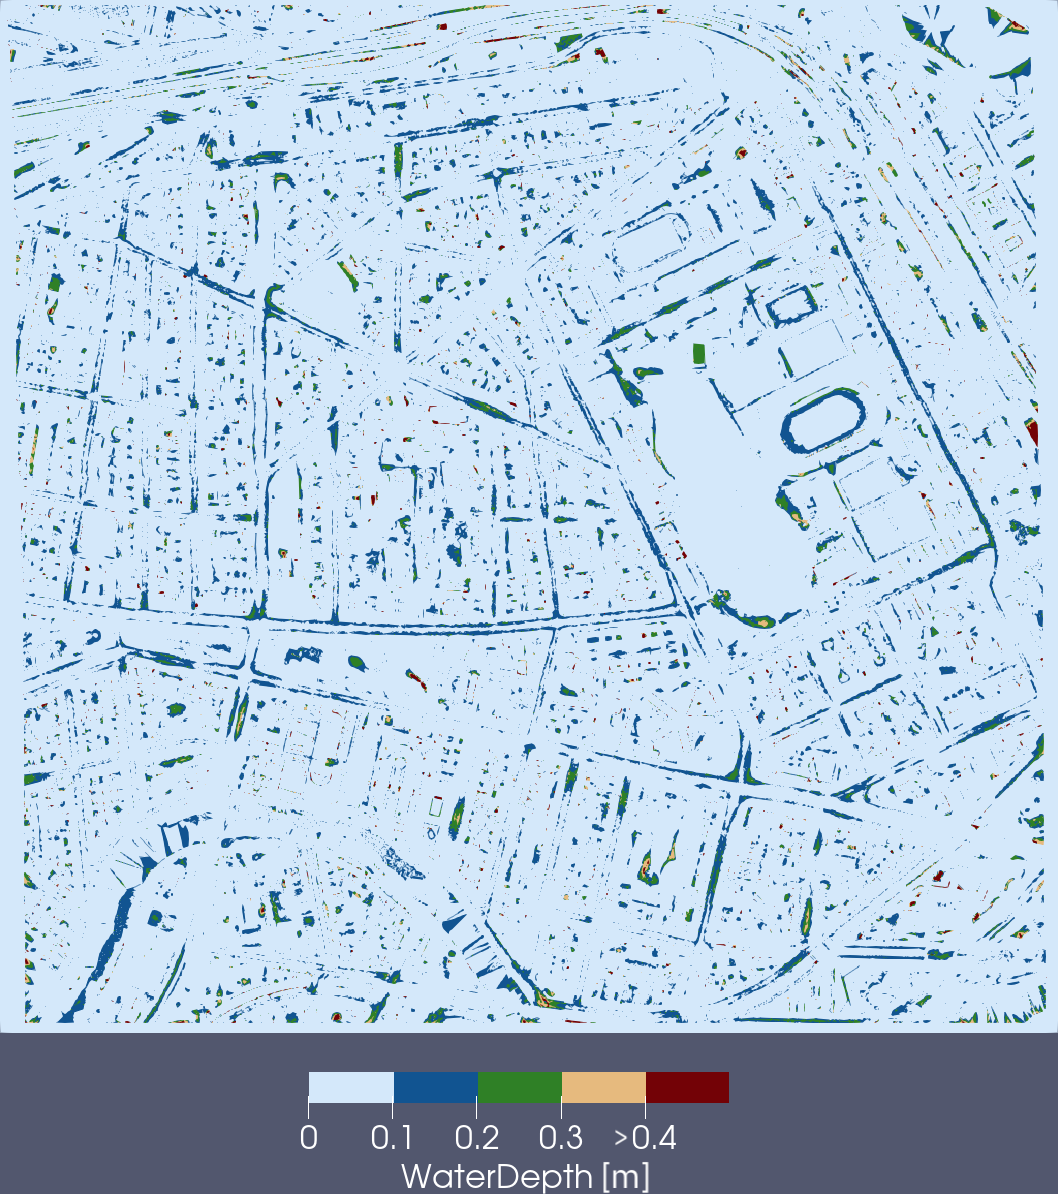
\includegraphics[width=\textwidth]{./img/moabit-1200s-lts-fo-d.png}
    \caption{
      \acrshort{lts} result for water depth
    }
    \label{fig:moabit-1200s-lts-fo-d}
  \end{subfigure}
  \hspace{0.5cm}
  \begin{subfigure}[t]{0.45\textwidth}
    \centering
    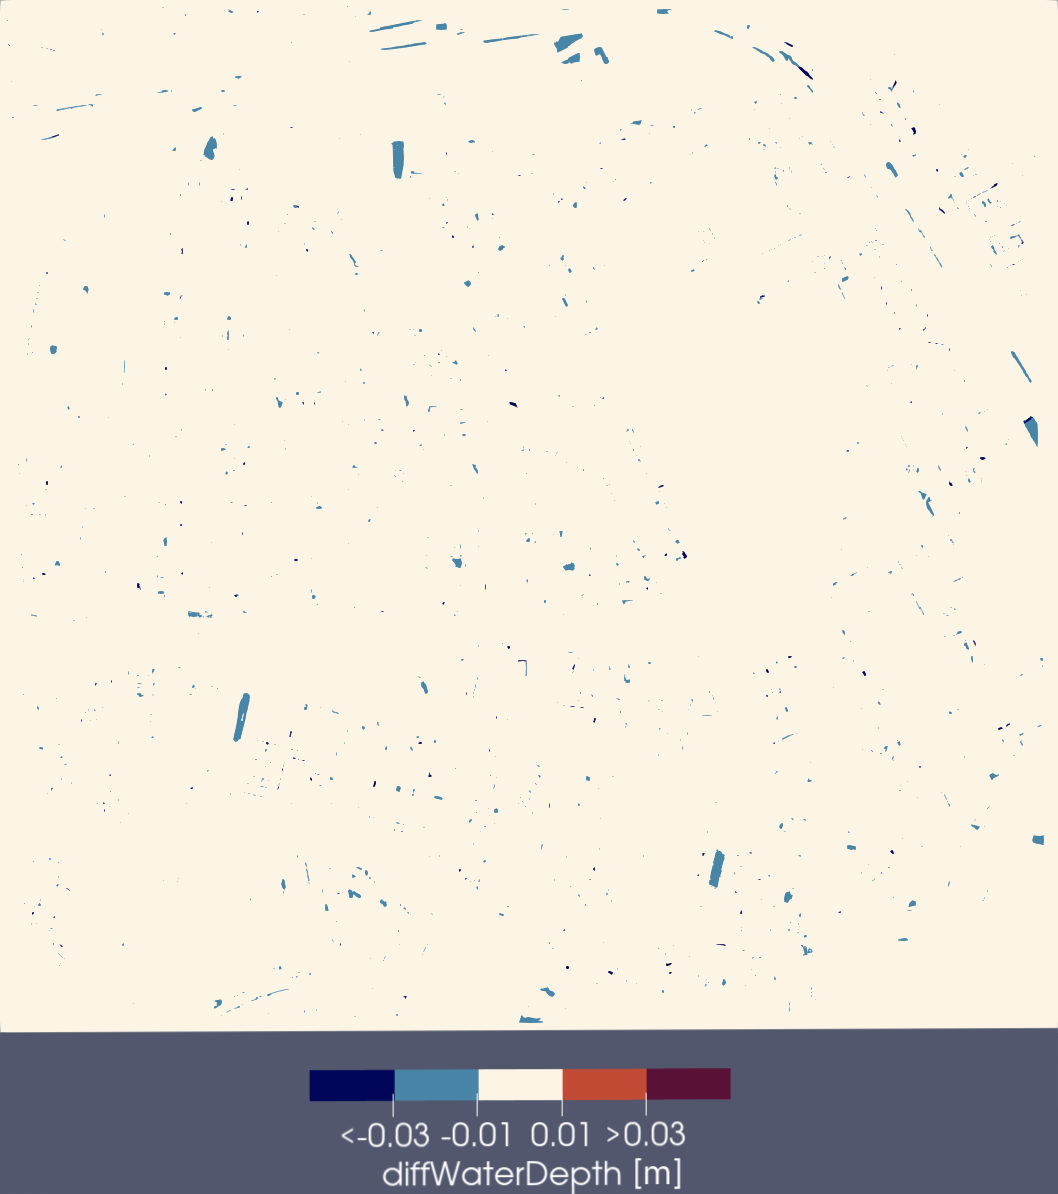
\includegraphics[width=\textwidth]{./img/moabit-1200s-lts-fo-diff.png}
    \caption{
      Difference of water depth between results obtained with \acrshort{lts} and \acrshort{gts} schemes
    }
    \label{fig:moabit-1200s-lts-fo-diff}

  \end{subfigure}
  \caption{Results of the practical case, simulated using first-order reconstruction,  
  $t = \SI{1200}{\second}$.}
  \label{fig:moabit-1200s-lts-fo-paraview}
\end{figure}

\autoref{fig:moabit-3600s-lts-fo-paraview} shows the resulting water depth of the \gls{lts} simulation using first-order reconstruction and a visualization of its error in comparison to the results obtained with \gls{gts}, at $t=\SI{3600}{\second}$.
Again, 
% the following analysis covers only first-order reconstruction, 
% as results obtained with \gls{tvd} showed large similarities.
only the results with first-order reconstruction are described here, as those obtained with \gls{tvd} are very similar in their characteristics.
Compared to \autoref{fig:moabit-1200s-lts-fo-diff}, the error regions have become more concentrated: there are fewer, but larger continuous regions. 
Again, most of them have an absolute error below $\SI{0.03}{\meter}$, just 81 of 1024000 cells (\SI{0.0079}{\percent}) show an absolute error greater than $\SI{0.05}{\meter}$,
and 13 (\SI{0.0013}{\percent}) deviate more than $\SI{0.10}{\meter}$. 
% The largest value is in a single cell at 
The three largest deviations are all $\sim\!\SI{0.23}{\meter}$.

\begin{figure} [p]
  \centering
  \begin{subfigure}[t]{0.45\textwidth}
    \centering
    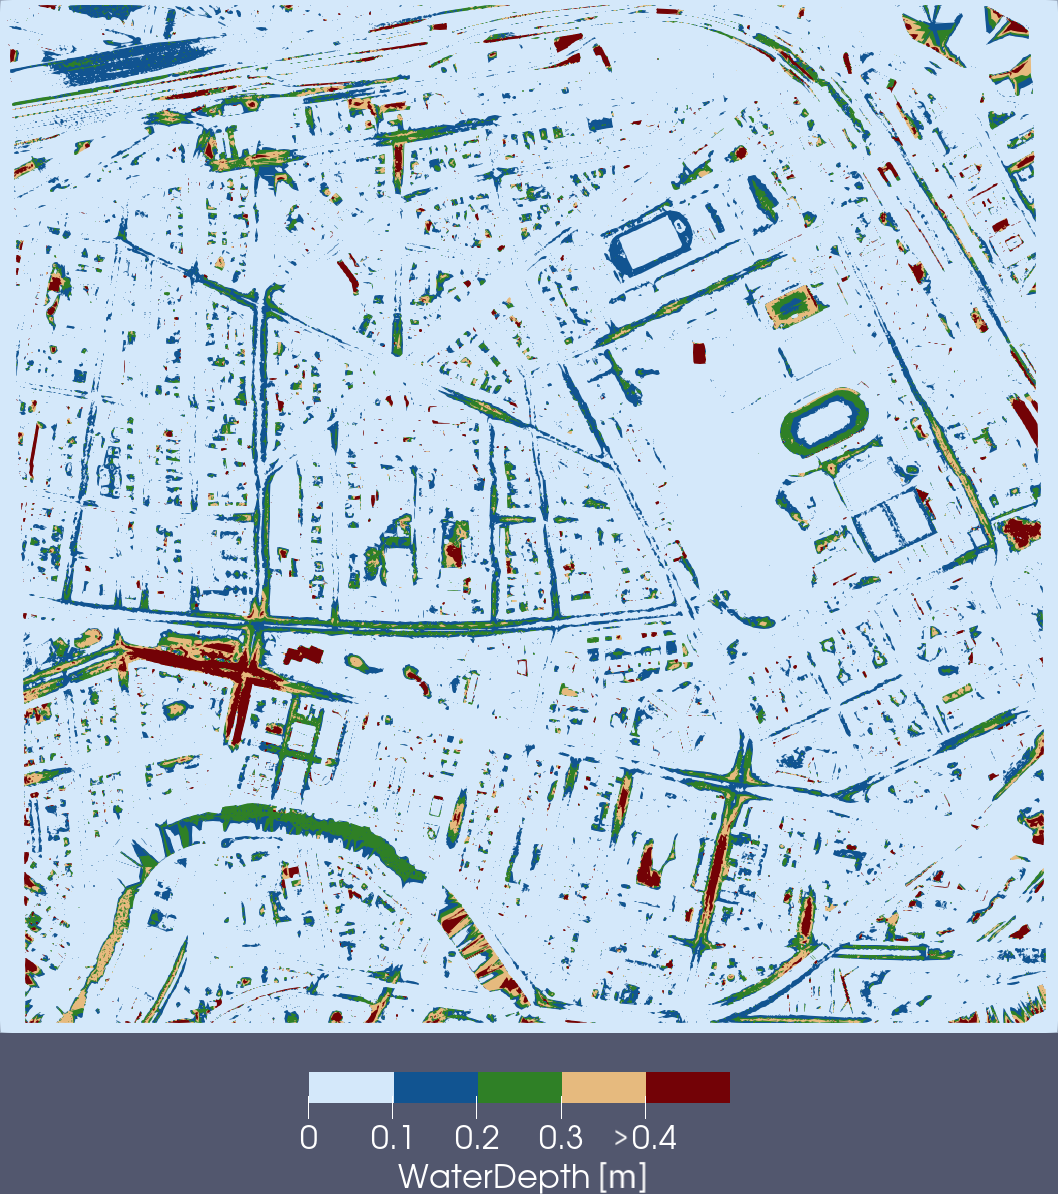
\includegraphics[width=\textwidth]{./img/moabit-3600s-lts-fo-d.png}
    \caption{
      \acrshort{lts} result for water depth
    }
    \label{fig:moabit-3600s-lts-fo-d}
  \end{subfigure}
  \hspace{0.5cm}
  \begin{subfigure}[t]{0.45\textwidth}
    \centering
    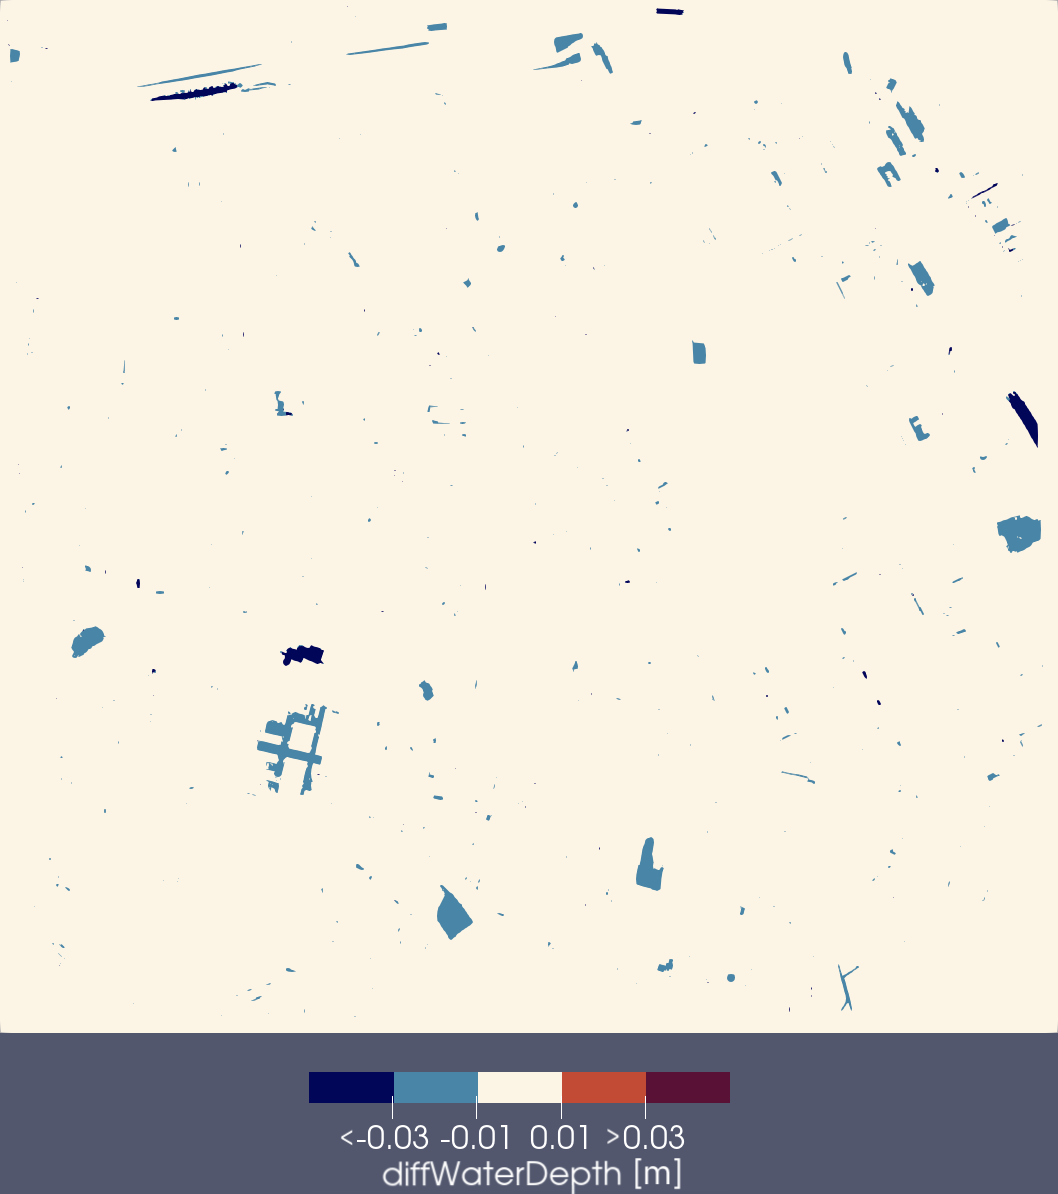
\includegraphics[width=\textwidth]{./img/moabit-3600s-lts-fo-diff.png}
    \caption{
      Difference of water depth between results obtained with \acrshort{lts} and \acrshort{gts} schemes.
    }
    \label{fig:moabit-3600s-lts-fo-diff}

  \end{subfigure}
  \caption{Results of the practical case, simulated using first-order reconstruction,  
  $t= \SI{3600}{\second}$.}
  \label{fig:moabit-3600s-lts-fo-paraview}
\end{figure}

\autoref{fig:moabit-error-plot} shows the development of the water depth's \gls{sae} of the \gls{lts} solution over time, for both first-order and \gls{tvd} reconstruction.
For both schemes, the \gls{sae} reaches a maximum value above $\SI{4000}{\meter}$ at $t=\SI{100}{\second}$, which is the first time at which results are exported, but stabilizes around $\SI{3695}{\meter}$ and $\SI{4260}{\meter}$, respectively, from $t=\SI{300}{\second}$ onward.

\begin{figure}[htbp]
  \centering
  \begin{tikzpicture}
  \begin{axis}[
      xlabel={$t \,[\si{\second}]$},
      ylabel={\acrshort{sae} $[\si\meter]$},
      xtick distance = 600,
      % ymin=-0.5,
      legend pos=south east,
      % legend style={at={(0.5,1.05)},anchor=south},
      % legend columns=2,
      % xmajorgrids=true,
      % grid style=loosely dashed,
      width=0.8\textwidth,
      height=7cm,
    ]
    % % analytical
    % \addplot [black, very thin, mark=none] 
    %   table [x=Time, y=WaterDepth, col sep=comma] {./graphs/real/moabit-fo-integrate.csv};
    % \addlegendentry{water depth $\int d_{\text{fo}} \,\differential A$}

    \addplot [CadetBlue, mark=x] 
      table [x=Time, y=abs_diffWaterDepth, col sep=comma] {./graphs/real/moabit-fo-integrate.csv};
    \addlegendentry{first-order}

    \addplot [lightgray, mark=o] 
      table [x=Time, y=abs_diffWaterDepth, col sep=comma] {./graphs/real/moabit-tvd-integrate.csv};
    \addlegendentry{\acrshort{tvd}}

    % \addplot [lightgray, mark=o] 
    %   table [x=Time, y=diffWaterDepth, col sep=comma] {./graphs/real/moabit-fo-integrate.csv};
    % \addlegendentry{difference $\int \Delta d \,\differential A$}
    
    % \legend{abs\_diffWaterDepth, diffWaterDepth}
  \end{axis}
\end{tikzpicture}
  \caption[
    Development of the water depth's \acrshort{sae} for first-order and \acrshort{tvd} reconstruction throughout simulation time.]{
    Development of the water depth's \acrshort{sae} of the \gls{lts} solution for first-order and \acrshort{tvd} reconstruction throughout simulation time.
  }
  \label{fig:moabit-error-plot}
\end{figure}

\subsubsection{Runtime Analysis}

\autoref{tab:real} shows the average runtime of 10 runs each for all three simulation durations, the relative difference between \gls{gts} and \gls{lts} runtimes and the \gls{ssc}.

\begin{table}[htb]
  \caption[Average runtime of 10 runs, \acrshort{rtr} and \acrshort{ssc} for the urban scenario.]
  {
    Average runtime of 10 runs, \acrfull{rtr} and \acrfull{ssc} for the urban scenario of each combination of \gls{gts}/\gls{lts} first-order/\gls{tvd} reconstruction.
  }
  \label{tab:real}
  \small
  \centering
  \sisetup{
  table-format=3.2,
}

\begin{tabular}{
  r
  % *{2}{S[round-mode=places,round-precision=1,table-space-text-post={\,s}]<{\,s}}
  % *{2}{S[round-mode=places,round-precision=1,table-format=2.1,table-space-text-post={\,\%}]<{\,\%}}
  % *{2}{S[round-mode=places,round-precision=1,table-space-text-post={\,s}]<{\,s}}
  % *{2}{S[round-mode=places,round-precision=1,table-format=2.1,table-space-text-post={\,\%}]<{\,\%}}
  *{2}{S[round-mode=places,round-precision=1]}
  *{2}{S[round-mode=places,round-precision=1,table-format=2.1]}
  *{2}{S[round-mode=places,round-precision=1]}
  *{2}{S[round-mode=places,round-precision=1,table-format=2.1]}
  }

  \toprule
   &  \multicolumn{4}{c}{first-order reconstruction} &  \multicolumn{4}{c}{\gls{tvd} reconstruction}                                                                                                                           \\
  \cmidrule(r){2-5} \cmidrule(r){6-9}

  % var0-base-dambreak_wet_0.6s_64x64_2000_gts_fo

                                      % &  \mc{\gls{gts}} & \mc{\gls{lts}} & \mc{\acrshort{rtr}} & \mc{\acrshort{ssc}} &  \mc{\gls{gts}} & \mc{\gls{lts}} & \mc{\acrshort{rtr}} & \mc{\acrshort{ssc}} \\
                                      & \mc{\gls{gts}\,[\si\second]} & \mc{\gls{lts}\,[\si\second]} & \mc{\acrshort{rtr}\,[\si\percent]} & \mc{\acrshort{ssc}\,[\si\percent]} & \mc{\gls{gts}\,[\si\second]} & \mc{\gls{lts}\,[\si\second]} & \mc{\acrshort{rtr}\,[\si\percent]} & \mc{\acrshort{ssc}\,[\si\percent]} \\
  \midrule
  $t = \SI{600}{\second}$  &  83.749         & 80.979         &  3.31               & 0.3187541463954003  &  179.49         & 147.96         &  17.57              & 24.642297705028334  \\
  $t = \SI{1200}{\second}$ &  357.29         & 350.39         &  1.93               & 3.881321355386417   &  560.28         & 521.83         &  6.86               & 18.201279123084777  \\
  $t = \SI{3600}{\second}$ &  2639.3         & 2057.1         &  22.06              & 32.24307031761723                                                                                   \\
  \bottomrule
\end{tabular}


\end{table}

As a first observation, the \gls{gts} runtimes in \autoref{tab:real} indicate that the global time step appears to decrease over the duration of the simulation: 
While it takes $\sim\!\SI{80}{\second}$ (\SI{180}{\second} with \gls{tvd}) to simulate the first \SI{600}{\second}, the next interval of the same length takes disproportionately longer, with (rounded) $\num{357} - \num{84} = \SI{273}{\second}$ using first-order and \SI{380}{\second} using \gls{tvd} reconstruction.
For first-order reconstruction, where such data is available, this trend continues: Here, the latter two thirds of the simulation take up \SI{97}{\percent} of the runtime.

The runtime reductions achieved by \gls{lts} over \gls{gts} differ greatly between the reconstruction schemes. 
In the first \SI{600}{\second}, a reduction of just \SI{3.3}{\percent} is obtained with first-order reconstruction. However, the \gls{ssc} amounts to just \SI{0.3}{\percent}, which contradicts previous results obtained in \autoref{sec:results-accuracy-analytical} and \textcite{crossley2003}, as runtime reduction exceeds the \gls{ssc}.
By contrast, a runtime reduction of \SI{17.6}{\percent} and a \gls{ssc} of \SI{24.64}{\percent}, is achieved with \gls{tvd} in the same period.
When considering up to \SI{1200}{\second}, the runtime reduction is reduced for both schemes, to $<\SI{2}{\percent}$ and $<\SI{7}{\percent}$, respectively. 
Similarly, the \gls{ssc} decreased to \SI{18.2}{\percent} for \gls{tvd}, or \SI{7.29}{\percent} if only inner blocks are considered.
However, the last two thirds of the simulation appear to benefit much more from using \gls{lts}, as here, and with first-order reconstruction, a runtime reduction of $>\SI{22}{\percent}$ was observed.

To further investigate this behavior, heatmaps showing the \gls{ssc} per block, are provided in 
Figures \ref{fig:heatmap-moabit-600s}--\ref{fig:heatmap-moabit-3600s}, with first order on the left and \gls{tvd} on the right. 
%
For short simulations of 10 minutes (\SI{600}{\second}), the \gls{ssc} diverges, depending on the utilized reconstruction scheme.
\autoref{fig:heatmap-moabit-600s-fo} represents the low overall \gls{ssc} of the first-order scheme
at this time. It does not show any noticeable local \gls{ssc} either.
In contrast, \autoref{fig:heatmap-moabit-600s-tvd} shows notably higher values ($\sim\!10-\SI{20}{\percent}$) in a very uniform distribution of scalar flux computations across the whole domain for the \gls{tvd} reconstruction, matching the higher overall \gls{ssc}.
However, it has been observed, that \gls{tvd} boundary blocks receive more scalar flux computations than inner blocks: 
when looking at all blocks, the \gls{ssc} amounts to \SI{24.64}{\percent}, as it is obtained per block, not per cell.
On the other hand, just \SI{16.12}{\percent} of inner block updates could be carried out as scalar flux computations.
The boundary blocks, which make up \SI{21.6}{\percent} (70 out of 324) of all blocks, distort the overall \acrlong{ssc}, as their \acrshort{ssc} amounts to \SI{55.1}{\percent}.
Due to their small size, they are not noticeable in \autoref{fig:heatmap-moabit-600s-tvd}.
Thus far, no explanation could be found for the divergence between reconstruction schemes and the differing behavior of boundary blocks.

In simulations of 20 minutes (\SI{1200}{\second}), both reconstruction schemes' runtime reduction decreases in comparison to first \SI{600}{\second}.
Both heatmaps in \autoref{fig:heatmap-moabit-1200s} show largely similar distributions of \gls{ssc} values, with small regions exhibiting relatively high \gls{ssc} values of $\sim\!40-\SI{50}{\percent}$. These regions are the same for both schemes.
% Other regions around them show  slightly larger values for the \gls{tvd} scheme in comparison to the first-order scheme.
Once more, the boundary and inner blocks of the \gls{tvd} scheme diverge: 
the overall \gls{ssc} amounts to \SI{18.2}{\percent} for \gls{tvd}, 
or \SI{7.3}{\percent}, if only inner blocks are considered. In contrast, the outer blocks' value of \SI{57.6}{\percent} even exceeds the previous value at $t=\SI{600}{\second}$.
This, again, cannot be explained by current results, as increases in the \gls{ssc} should cause runtime reduction to increase in return.

Finally, when considering a full hour of simulated time,
the \gls{ssc} increases further, exceeding all previous values. 
\autoref{fig:heatmap-moabit-3600s} shows a much wider distribution of \gls{ssc} values between regions: 
Both higher \gls{ssc} per block and more blocks with high \gls{ssc} are achieved.
The vast majority of blocks exhibit a \gls{ssc} $>\SI{10}{\percent}$ and several clusters of high \gls{ssc} values can be identified.
Blocks with large \gls{ssc} values at $t=\SI{1200}{\second}$ maintain this status, 
but with increased values of $\sim\!80-\SI{90}{\percent}$ and several of these form centers of such clusters.
The increased range of local \gls{ssc} is likely due to the much more heterogeneous water depth, shown in \autoref{fig:moabit-3600s-lts-fo-d}, as it has a large impact on the size of the local time step.

\begin{figure} [hb]
  \centering
  \begin{subfigure}[t]{0.45\textwidth}
    \centering
    \includegraphics[width=\textwidth]{../typst/heatmaps/real/moabit_600s_lts_fo.pdf}
    \caption{
      First-order reconstruction
    }
    \label{fig:heatmap-moabit-600s-fo}
  \end{subfigure}
  \hspace{0.5cm}
  \begin{subfigure}[t]{0.45\textwidth}
    \centering
    \includegraphics[width=\textwidth]{../typst/heatmaps/real/moabit_600s_lts_tvd.pdf}
    \caption{
      \acrshort{tvd} reconstruction
    }
    \label{fig:heatmap-moabit-600s-tvd}

  \end{subfigure}
  \caption{
    Heatmap for scalar/full flux computations, at time $t = \SI{600}{\second}$ for the urban scenario.
    }
  \label{fig:heatmap-moabit-600s}
\end{figure}

\begin{figure} [p]
  \centering
  \begin{subfigure}[t]{0.45\textwidth}
    \centering
    \includegraphics[width=\textwidth]{../typst/heatmaps/real/moabit_1200s_lts_fo.pdf}
    \caption{
      First-order reconstruction
    }
    \label{fig:heatmap-moabit-1200s-fo}
  \end{subfigure}
  \hspace{0.5cm}
  \begin{subfigure}[t]{0.45\textwidth}
    \centering
    \includegraphics[width=\textwidth]{../typst/heatmaps/real/moabit_1200s_lts_tvd.pdf}
    \caption{
      \acrshort{tvd} reconstruction
    }
    \label{fig:heatmap-moabit-1200s-tvd}

  \end{subfigure}
  \caption{
    Heatmap for scalar/full flux computations, at time $t = \SI{1200}{\second}$ for the urban scenario.
    }
  \label{fig:heatmap-moabit-1200s}
\end{figure}

\begin{figure} [p]
  \centering
  \includegraphics[width=0.45\textwidth]{../typst/heatmaps/real/moabit_3600s_lts_fo.pdf}
  \caption{
    Heatmap for scalar/full flux computations, at time $t = \SI{3600}{\second}$ for the urban scenario, computed using first-order reconstruction.
  }
  \label{fig:heatmap-moabit-3600s}
\end{figure}

\FloatBarrier
\newpage
\FloatBarrier
\subsection{Stability}\label{sec:results-ugly}

Within the process of implementing the \gls{frozen-block-LTS} scheme, additional test cases have been run, e.g., to gain insights into stability and mass conservation of the scheme.
One of these is a variation of the \gls{1D} wet dam break used above:
free outflow was disabled at all boundaries to maintain 
the total water volume, 
and the simulation duration was extended to \SI{120}{\second}.
Mesh and block sizes were set to $400 \times 150$ and $8 \times 8$ cells, respectively.
Other parameters were adopted from the base configuration used in \autoref{sec:results-benchmarks}.
The extended duration allowed the wave to reach the downstream boundary and be reflected.
\autoref{fig:tvd-checker-boarding} shows a three-dimensional visualization of the water surface at $t=\SI{110}{\second}$ -- after the reflection of the wave, which occours at $t\sim\SI{35}{\second}$.
While the results of the first-order scheme show a smooth surface, the results of the \gls{tvd} scheme show instabilities in the form of checker-boarding.
The modification described in \autoref{sec:criterion-mod} has reduced this behavior, but it could not be fully prevented.

While providing overall good stability, there exist combinations of schemes and boundary conditions, under which the proposed \gls{lts} scheme in its current form does not reach the same level of stability as \gls{hms}' \gls{gts} scheme.

\begin{figure}[H]
  \centering
  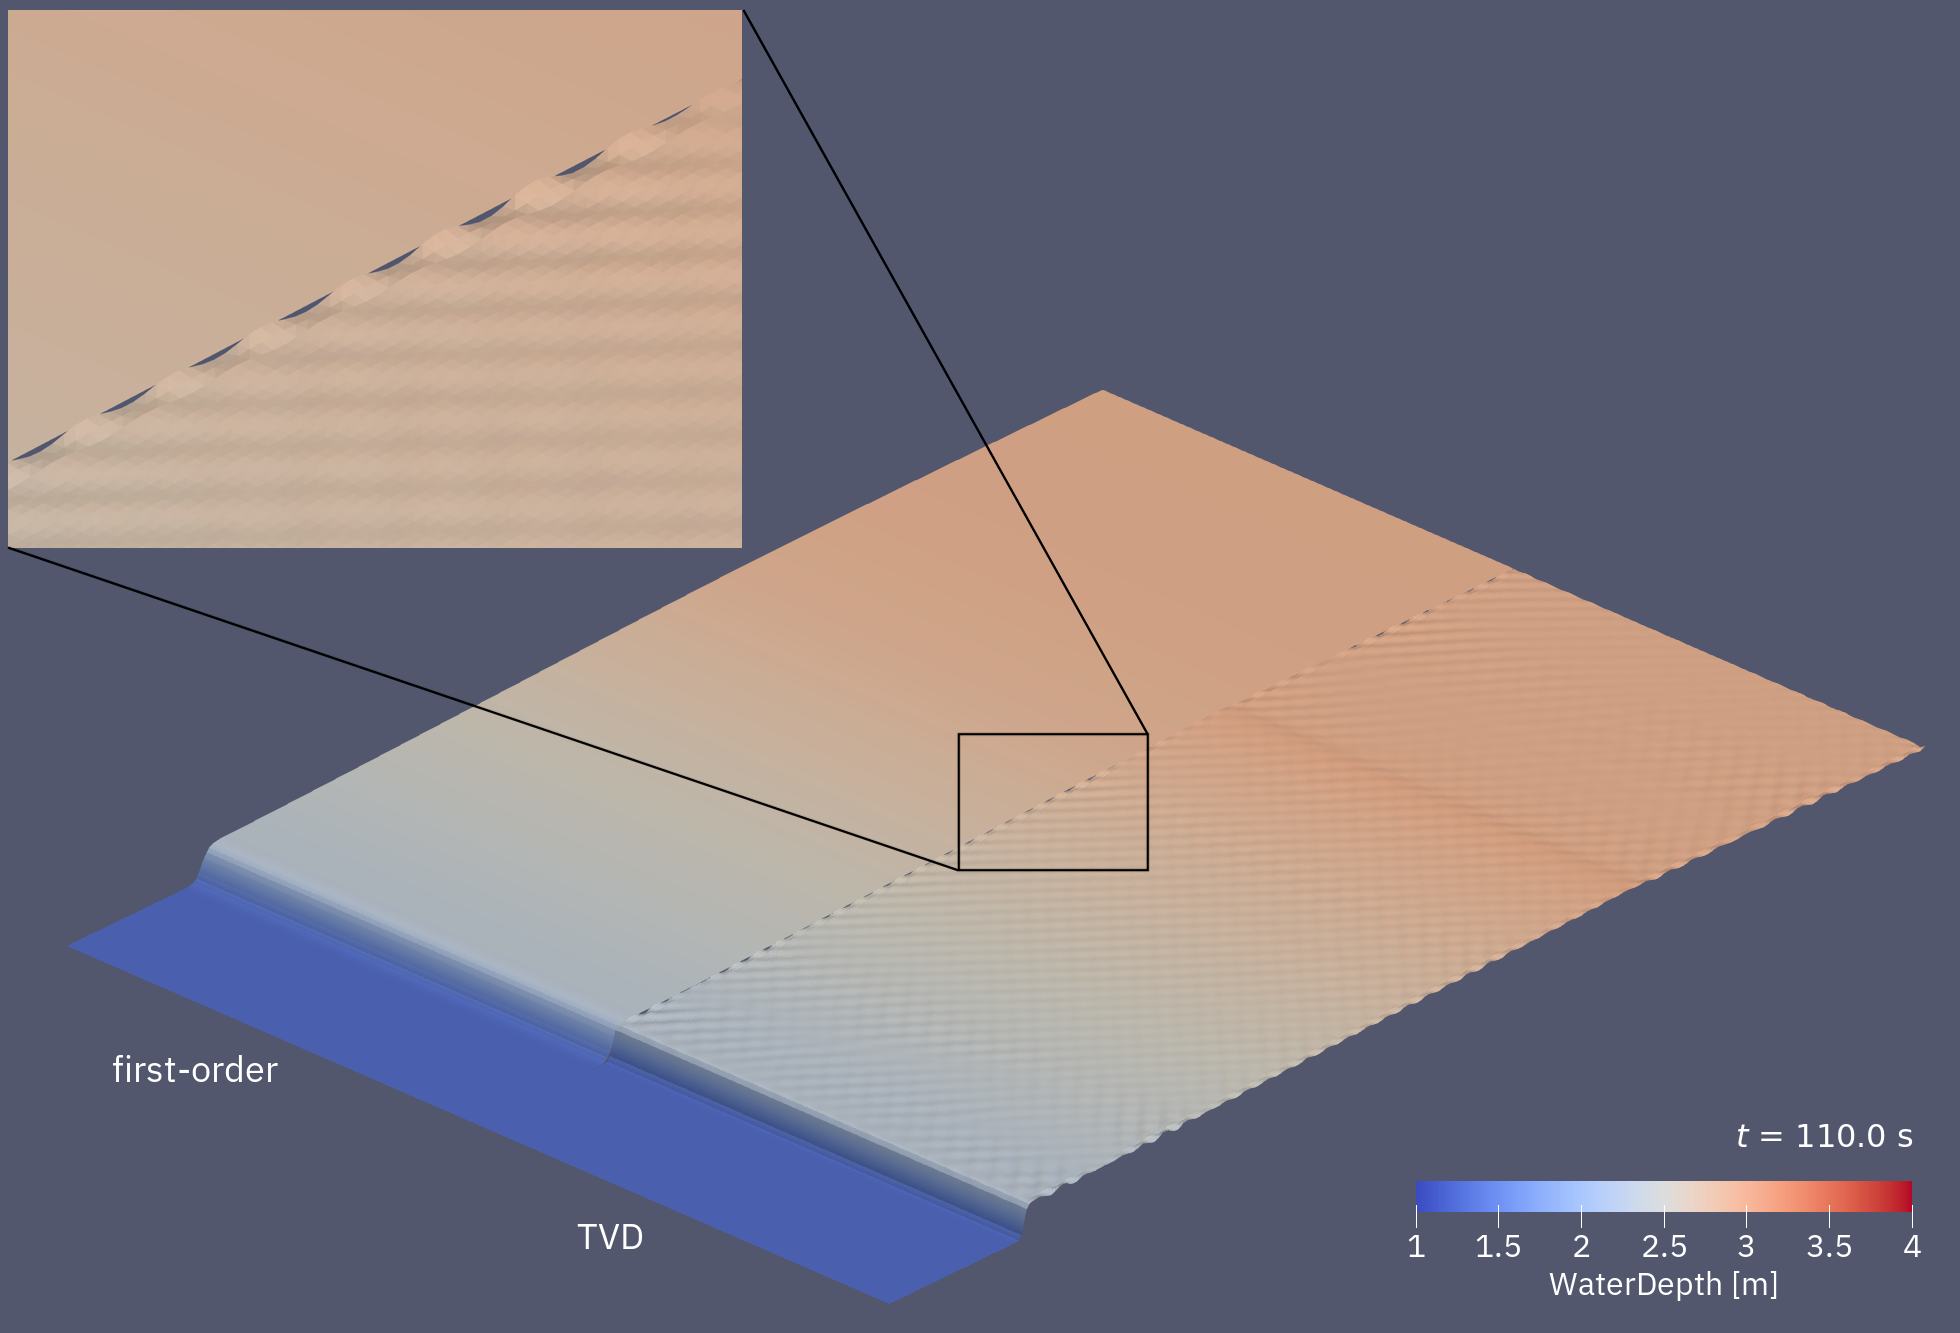
\includegraphics[width=\textwidth]{./img/cons_dambreak-t110.png}
  \caption
  [Water surfaces of the wet dam break case without outflow]
  {Water surfaces of the wet dam break case without outflow at $t=\SI{110}{\second}$. The upper right corner shows a maginified portion of the mesh. }\label{fig:tvd-checker-boarding}
  \vspace{-1cm}
\end{figure}